\documentclass[14pt,a4paper]{article}
\usepackage[14pt]{extsizes}
\usepackage[left=1.5cm, right=1.5cm, top=1.5cm, bottom=1.5cm]{geometry}
\usepackage[utf8]{inputenc}
\usepackage[T2A]{fontenc}
\usepackage[english, russian]{babel}
\usepackage{amsmath,amsfonts,amssymb,amsthm,mathtools} 
\usepackage{amsfonts}
\usepackage{amssymb}
\usepackage{titleps}
\usepackage{hyperref}
\usepackage{float}
\usepackage{graphicx}
\usepackage{multirow}
\usepackage{hhline}
\usepackage{wrapfig}
\usepackage{tikz}
\usepackage{pgfplots}
\usepackage{xcolor}
\usepackage{subfig}
\usepackage{upgreek}

\newcommand{\w}[1]{\text{#1}}
\newcommand{\und}[1]{\underline{#1}}
\newcommand{\img}[3]{
	\begin{figure}[H]
	\begin{center}
	\includegraphics[scale=#2]{#1}
	\end{center}
	\begin{center}
 	\textit{#3}
	\end{center}
	\end{figure}
}
\newcommand{\aw}[1]{
	\begin{center}
	\textit{#1}
	\end{center}
	\n
}
\newcommand{\be}[1]{
	\begin{center}
	\boxed{#1}
	\end{center}
}
\newcommand{\beb}[1]{
	\begin{equation}
	\boxed{#1}
	\end{equation}
}
\newcommand{\eb}[1]{
	\begin{equation}
	#1
	\end{equation}
}
\newcommand{\n}{\hfill \break}
\newcommand{\x}{\cdot}

\begin{document}
\section*{Работа 3.2.5}	
	\section*{Свободные и вынужденные колебания в электрическом контуре}
	\subsection*{Андрей Киркича, Б01-202, МФТИ}
	\n
	\textbf{В работе используются: }
осциллограф; генератор сигналов специальной формы; магазин сопротивления; магазин емкости; магазин индуктивности; соединительная коробка с шунтирующей емкостью; соединительные одножильные и коаксиальные провода.

\section*{Экспериментальная установка}
Картина колебаний напряжения на емкости наблюдается на экране двухканального осциллографа. Для возбуждения затухающих колебаний используется генератор сигналов специальной
формы. Сигнал с генератора поступает через конденсатор $C_1$ на вход колебательного контура. Данная емкость необходима, чтобы выходной импеданс генератора был много меньше импеданса колебательного контура и не влиял на процессы, проходящие в контуре.

\begin{figure}[H]
\centering
\subfloat[Схема установки для исследования вынужденных колебаний]{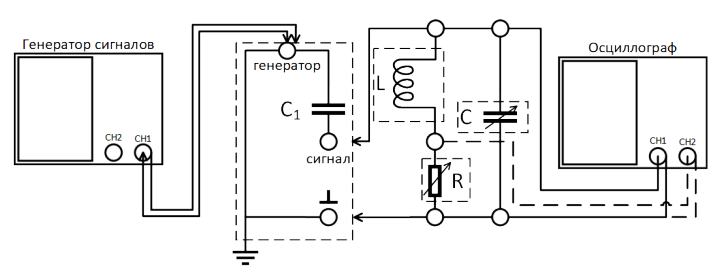
\includegraphics[width=0.45\textwidth]{1.png}}
\qquad
\subfloat[Схема установки для исследования АЧХ и ФЧХ]{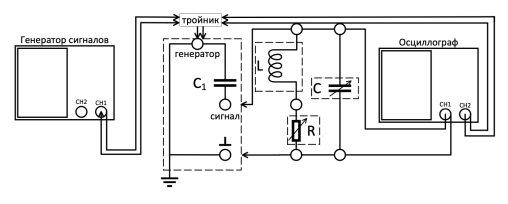
\includegraphics[width=0.45\textwidth]{2.png}}
\end{figure}
\n
При изучении свободно затухающих колебаний генератор специальных сигналов на вход колебательного контура подает периодические короткие импульсы, которые заряжают конденсатор $C$. За время между
последовательными импульсами происходит разрядка конденсатора через резистор и катушку индуктивности. Напряжение на конденсаторе $U_C$ поступает на вход канала 1(X) электронного осциллографа. Для наблюдения фазовой картины затухающих колебаний на канал 2(Y) подается напряжение с резистора $R$ (пунктирная линия на
схеме установки), которое пропорционально току $I$.
\n\n
При изучении возбужденных колебаний на вход колебательного контура подается синусоидальный сигнал. С помощью осциллографа возможно измерить зависимость амплитуды возбужденных колебаний в зависимости от частоты внешнего сигнала, из которого возможно определить добротность колебательного контура. Альтернативным способом расчета добротности контура является определение декремента затухания по картине установления возбужденных колебаний. В этом случае генератор сигналов используется для подачи цугов синусоидальной формы.

\section*{Выполнение работы}
\subsection*{Измерение периодов свободных колебаний}

На генераторе предварительно была установлена последовательность импульсов со следующими параметрами: длительность импульсов - 10 мкс, частота повторения - 100 Гц, амплитуда сигнала - 20 В. На магазине сопротивлений было установлено минимальное значение, на магазине индуктивностей - $L = 100$ мГн (во время проведения работы это значение оставалось постоянным), на магазине емкостей - $C = 0$ мкФ. На экране осциллографа была получена картина свободных затухающих колебаний.
\n\n
Был измерен период затухающих колебаний $T = (67,0 \pm 1,0)$ мкс. По этому значению была найдена нулевая ёмкость колебательного контура:
\[ C_0 = \frac{T^2}{4 \pi^2 L} = (1,1 \pm 0,2) \text{ нФ.} \]
Изменяя ёмкость (по курбелям) от 0 до 9 нФ, мы провели измерения периодов:
\begin{table}[H]
\centering
\begin{tabular}{|r|r|r|r|r|r|}
\hline
$C$, нФ & 1 & 3 & 5 & 7 & 9 \\ \hline
$T_{\text{эксп}}$, мкс & $110 \pm 9$ & $127 \pm 9$ & $142 \pm 9$ & $154 \pm 9$ & $169 \pm 9$ \\ \hline
$T_{\text{теор}}$, мкс & $108 \pm 7$ & $126 \pm 7$ & $141 \pm 7$ & $153 \pm 7$ & $166 \pm 7$ \\ \hline
\end{tabular}
\end{table}
\n
Учитывая, что $R_{\Sigma} = R + R_{L}$, построим график:
\begin{center}
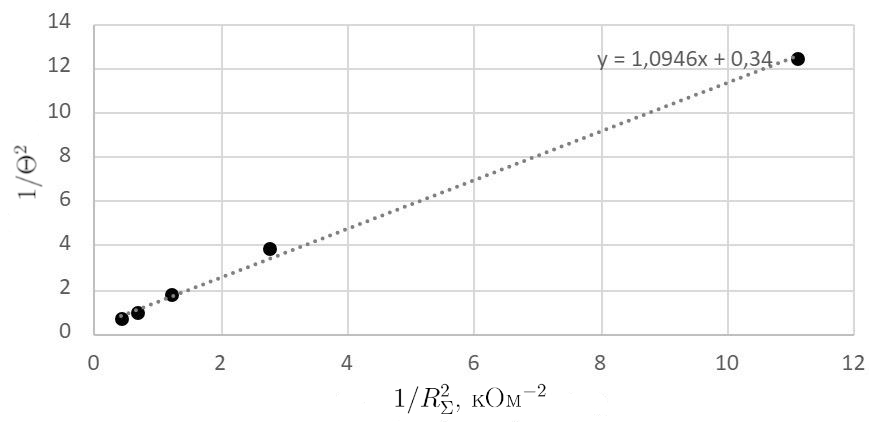
\includegraphics[scale=2]{6.jpg}
\end{center}
\n
Как видно из графика, зависимость является линейной, что подтверждается теоретической справкой.
\subsection*{Критическое сопротивление и декремент затухания}
Ёмкость $C^*$, при которой собственная частота колебаний составляет $\nu_0 = 6,5$ кГц:
\[ C^* = \frac{1}{4 \pi^2 L \nu_0^2} = (6,1 \pm 0,6) \text{ нФ,} \]
и критическое сопротивление контура:
\[ R_{\text{крит}} = 2\sqrt{\frac{L}{C^*}} = (7,5 \pm 0,3) \text{ кОм.} \]
На магазине емкостей было установлено значение $0,007$ мкФ, близкое к $C^*$. Увеличивая сопротивление $R$ от $0$ до $R_{\text{крит}}$, мы определили сопротивление, при котором колебательный режим переходит в апериодический: $R_{\text{апер}} = 4$ кОм.
\begin{wrapfigure}{r}{0.5\textwidth}
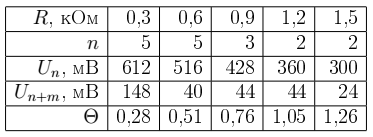
\includegraphics[scale=3]{tab1.png}
\vspace{-2cm}
\end{wrapfigure}
Затем мы устанавливали сопротивления в интервале $(0,05 - 0,25)R_{\text{крит}}$ и для каждого значения рассчитывали логарифмический декремент затухания по формуле: $\Theta = \frac{1}{n}\ln \frac{U_{m}}{U_{n + m}}$, где $n$ - целое число периодов, разделяющее максимумы.
\n\n
Для максимального и минимального значений $\Theta$ были найдены добротности:
\[ Q_{min} = \pi / \Theta_{min} = 11,22 \pm 0,07, \qquad \qquad Q_{max} = \pi / \Theta_{max} = 2,49 \pm 0,09. \]
\subsection*{Свободные колебания на фазовой плоскости}
\begin{wrapfigure}{l}{0.5\textwidth}
\vspace{-0.5cm}
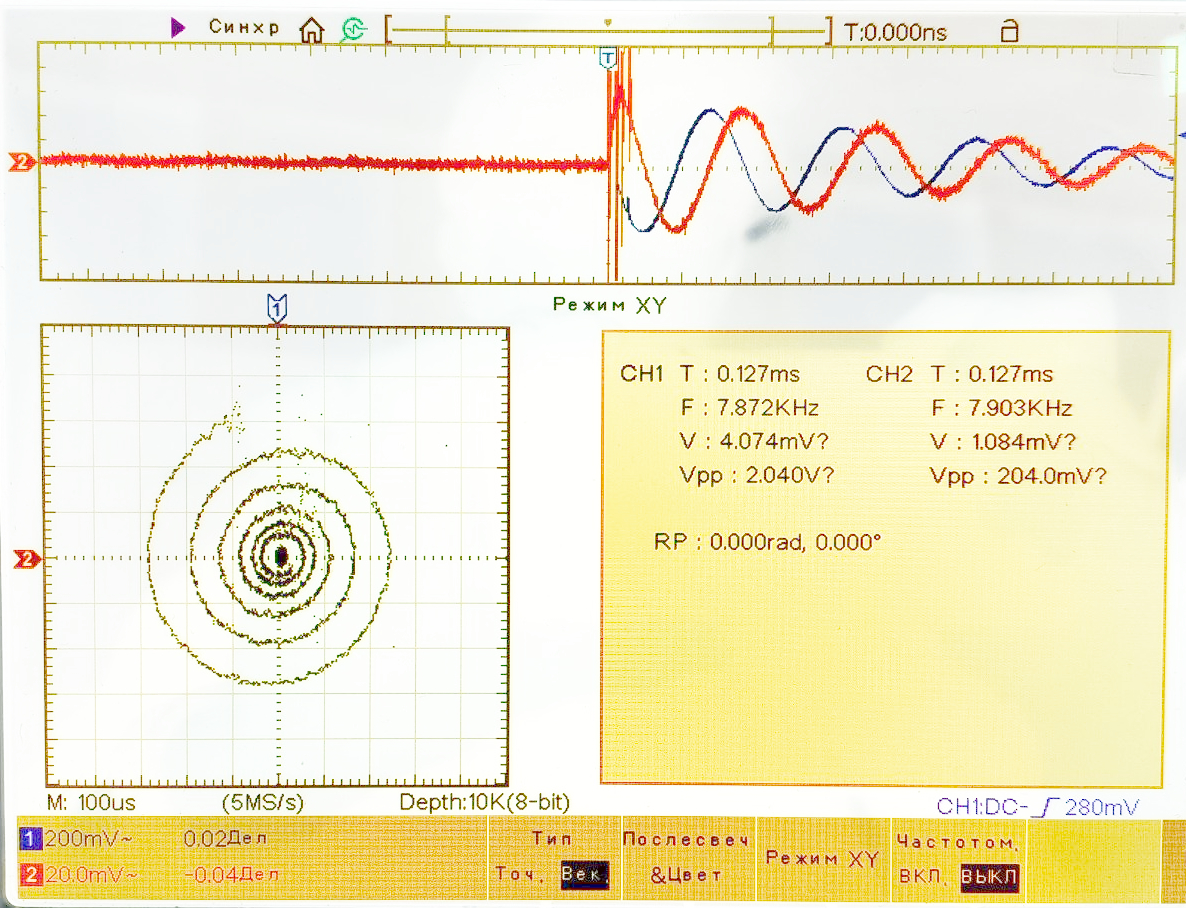
\includegraphics[scale=0.2]{3.jpg}
\vspace{-40pt}
\end{wrapfigure}
На магазине сопротивлений было установлено значение $R = 0,3$ кОм, на канал 2(Y) осциллографа подана величина падения напряжения с резистора. Переключив осциллограф в режим XY, мы получили картину затухающих колебаний на фазовой плоскости. Она представляет из себя спираль, сходящуюся к центру.
\n
\subsection*{Резонансные кривые}
В этом пункте работы мы установили $C = C^*$, $R = 0,3$ кОм, подали сигнал с генератора одновременно на колебательный контур и канал 2 осциллографа. При частотах, близких к резонансным, наблюдался устойчивый синусоидальный сигнал, амплитуда колебаний при этом стремилась к максимуму. Была найдена резонансная частота: $\nu_{\text{рез}} = 6,5$ кГц.
\n\n
АЧХ и ФЧХ контура:
\begin{figure}[H]
\centering
\subfloat[Амплитудно-частотная характеристика]{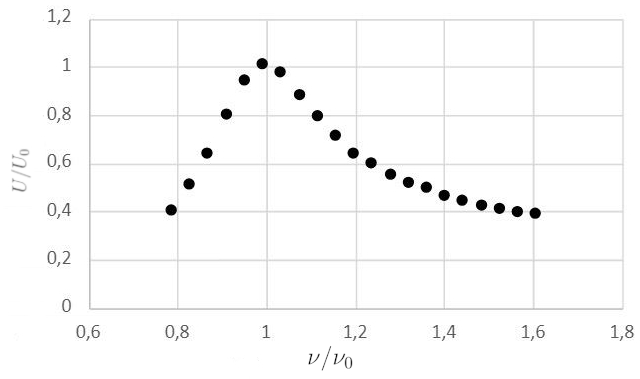
\includegraphics[width=0.45\textwidth]{5.jpg}}
\qquad
\subfloat[Фазово-частотная характеристика]{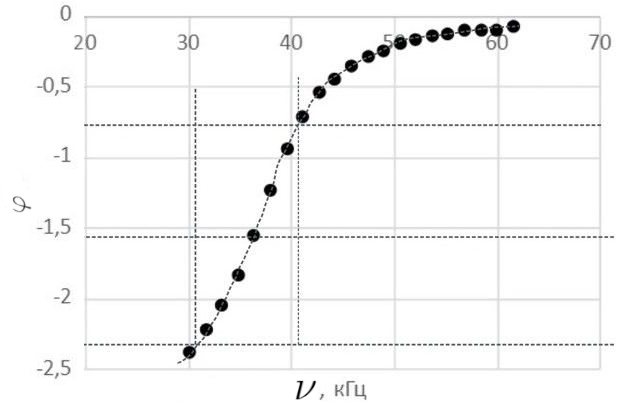
\includegraphics[width=0.45\textwidth]{7.jpg}}
\end{figure}
\section*{Заключение}
По данным, полученным в ходе экспериментов, были рассчитаны добротности контура при разных значениях сопротивления, получена картина затухающих колебаний на фазовой плоскости, а также построены амплитудно-частотная и фазово-частотная характеристики.

\section*{Литература}
\n
1. Никулин М.Г., Попов П.В., Нозик А.А., и др. Лабораторный практикум по общей физике: учеб. пособие. В трёх томах. Т. II. Электричество и магнетизм. - 2-е издание. М.: МФТИ, 2019\n
2. Сивухин Д. В. Общий курс физики. Учеб. пособие: Для вузов. Т. III. Электричество. - 6-е издание. М.: ФИЗМАТЛИТ, 2019
\end{document}